\documentclass[sigconf]{acmart}
\usepackage[utf8]{inputenc}
\usepackage[english]{babel}
\usepackage{lmodern}
\usepackage[T1]{fontenc}    
\usepackage{csquotes}

\usepackage{color}
\usepackage{subcaption}

\usepackage{hyperref}

\usepackage{amssymb}
\usepackage{amsmath}
\DeclareMathOperator*{\argmin}{arg\,min\,}
\DeclareMathOperator*{\argmax}{arg\,max\,}
\DeclareMathOperator{\sign}{sign}
\DeclareMathOperator{\loss}{loss}
\DeclareMathOperator{\softmax}{softmax}\DeclareMathOperator{\softplus}{softplus}

\DeclareMathOperator{\EX}{\mathbb{E}}% expected value

\newcommand{\myvec}[1]{\boldsymbol{#1}}
\newcommand{\minimize}{\text{minimize}}
\newcommand{\optimize}[4]{\begin{aligned}
& \underset{#2}{#1}
& & #3 \\
& \text{subject to}
& & #4
\end{aligned}}
\usepackage{natbib}
\setcitestyle{square, comma, numbers,sort&compress, super}

\usepackage{tikz}
\usetikzlibrary{positioning}
\usepackage{tikz-qtree}
\usetikzlibrary{arrows, calc, decorations.pathreplacing, angles, quotes, positioning}
\usetikzlibrary{shapes.geometric}
\usetikzlibrary{chains}

% configure acm template to a minimalistic version
\setcopyright{none}
\settopmatter{printccs=false, printacmref=false, printfolios=false}
\renewcommand\footnotetextcopyrightpermission[1]{} % removes footnote with conference information in first column
\pagestyle{plain} % removes running headers

\widowpenalty
\clubpenalty

\begin{document}
% Title portion
\title{InformatiCup 2019}

\author{Jonas Möller}
\affiliation{%
	\institution{TU Braunschweig}
}
\email{jo.moeller@tu-braunschweig.de}

\author{Lukas Pirch}
\affiliation{%
	\institution{TU Braunschweig}
}
\email{l.pirch@tu-braunschweig.de}

\maketitle
\section{Introduction}

\begin{enumerate}
\item Thema motivieren
\begin{enumerate}
\item Was ist ML?
\item Wofür wird ML benutzt?
\item Was sind Adversarial Examples (Irrbilder)?
\item Gefahr durch Adversarial Examples?
\end{enumerate}
\item Stand der Forschung erklären
\item Gliederung (?)
\end{enumerate}


Context: Self driving cars which automatically detect and classify traffic signs.
Threat: Patterns (e.g. on the back of a lorry) might be classified as a traffic sign and leads to a wrong and potentially dangerous response of the car.

\begin{enumerate}
\item herausarbeiten, dass es um digitale adversarial samples geht
(i.e. relativ kleiner input 64x64 und pixelgenaue veränderungen werden betrachten)
in kontrast zu: \cite{eykholt2018robust}
\end{enumerate}

Find images (Irrbilder) that do not look like traffic signs to a human observer,
but are recognized with a confidence of >90\% as a traffic sign by the neural network.

This corresponds to the current scientific research direction of adversarial examples.
These are images which are specifically created by an attacker with the intention of tricking the machine learning system into misclassifying.

The neural network under attack is available via a web interface,
which reports the top five most-likely classes and their confidences for a given image.
Additionally, we are given the information that the remote model has been trained on the GTSRB dataset.
This equates to Oracle access ($X \rightarrow Y$) and Training data ($T$) knowledge \cite{papernot2016limitations}.

Adversarial Examples are an active research direction and though there exist a plethora of attacks,
it's neither clearly established why adversarial examples exist nor how to effectively defend against them.
One of the most prominent projects for benchmarking defenses is the CleverHans project where a lot of state-of-the-art attacks are included \cite{papernot2016cleverhans}.

% Damn it I had something for this
% Something something Source-Target misclassifcation 
%!TEX root = paper.tex"`

\section{Background}\label{sec:background}

\begin{figure}
\centering
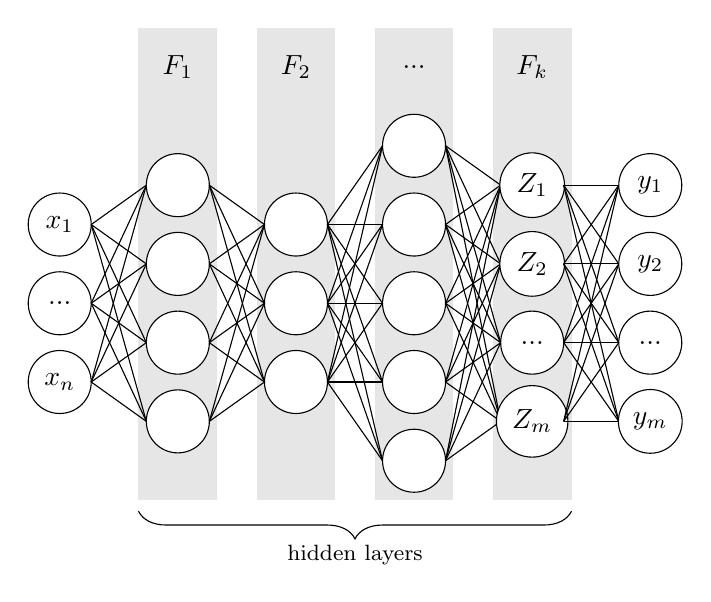
\begin{tikzpicture}[yscale=-1]
\tikzset{neuron/.style={
    shape=circle,
    fill=white,
    draw,
    minimum size=0.8cm
}}

%\draw[step=1cm,gray,very thin,fill=white] (0,0) grid (8,6);

\fill[opacity=0.2,fill=gray] (1,-0.5) rectangle (2,5.5);

\fill[opacity=0.2,fill=gray] (2.5,-0.5) rectangle (3.5,5.5);

\fill[opacity=0.2,fill=gray] (4,-0.5) rectangle (5,5.5);

\fill[opacity=0.2,fill=gray] (5.5,-0.5) rectangle (6.5,5.5);

\node[neuron] at (0, 2) {$x_1$};
\node[neuron] at (0, 3) {...};
\node[neuron] at (0, 4) {$x_n$};

\foreach \x in {1,...,3}{
	\draw (0.4, \x+1) -- (1.1,1.5);	\draw (0.4, \x+1) -- (1.1,2.5);
	\draw (0.4, \x+1) -- (1.1,3.5);
	\draw (0.4, \x+1) -- (1.1,4.5);
}

\node[] at (1.5, 0) {$F_1$};
\foreach \x in {2,...,5}{
	\node[neuron] at (1.5, \x-0.5) {};
	\draw (1.9, \x-0.5) -- (2.6,2);
	\draw (1.9, \x-0.5) -- (2.6,3);
	\draw (1.9, \x-0.5) -- (2.6,4);
}

\node[] at (3, 0) {$F_2$};
\foreach \x in {2,...,4}{
	\node[neuron] at (3, \x) {};
	\draw (3.4, \x) -- (4.1,1);	\draw (3.4, \x) -- (4.1,2);
	\draw (3.4, \x) -- (4.1,3);
	\draw (3.4, \x) -- (4.1,4);
	\draw (3.4, \x) -- (4.1,5);
}

\node[] at (4.5, 0) {...};
\foreach \x in {1,...,5}{
	\node[neuron] at (4.5, \x) {};
	\draw (4.9, \x) -- (5.6,1.5);	\draw (4.9, \x) -- (5.6,2.5);
	\draw (4.9, \x) -- (5.6,3.5);
	\draw (4.9, \x) -- (5.6,4.5);
}

\draw [decorate,decoration={brace,amplitude=10pt,mirror,raise=4pt},yshift=0pt]
(1,5.5) -- (6.5,5.5) node [black,midway,yshift=-0.7cm] {\footnotesize hidden layers};

\node[] at (6, 0) {$F_k$};
\foreach \x in {1,...,2}:
	\node[neuron] at (6, \x+0.5) {$Z_\x$};
\node[neuron] at (6, 3.5) {...};
\node[neuron] at (6, 4.5) {$Z_m$};

\foreach \x in {1,...,4}{
	\draw (6.4, \x + 0.5) -- (7.1,1.5);
	\draw (6.4, \x + 0.5) -- (7.1,2.5);
	\draw (6.4, \x + 0.5) -- (7.1,3.5);
	\draw (6.4, \x + 0.5) -- (7.1,4.5);
}

\foreach \x in {1,...,2}:
	\node[neuron] at (7.5, \x+0.5) {$y_\x$};
\node[neuron] at (7.5, 3.5) {...};
\node[neuron] at (7.5, 4.5) {$y_m$};
\end{tikzpicture}
\caption{Visualization of a neural network}
\label{fig:neuralnetwork}
\end{figure}

This section provides the general background knowledge required to understand the remainder of this paper.
In addition, the basic notation which is going to be used later is defined.
A reader familiar with the domain of adversarial machine learning is suggested to continue reading at Subsection~\ref{sec:threatmodel}.

\subsection{Deep Neural Networks}\label{subsec:dnn}
Deep neural networks (DNNs) are a form of machine learning algorithms based on a concept loosely analogous to the human brain.
On a conceptual level, DNNs take a vector of numbers as an input and assign it a output vector which represents the probability for each class which has been considered during training.
Thus, real-world input objects need to be transformed to a so called \enquote{feature space}, their mathematical abstraction that can be passed to the DNN.
In the context of image recognition, this relates to taking each input pixel's color channel as an input feature.
Having a look on the inner structure, neural networks consist of a set of nodes (\enquote{neurons}), which are organized in successive layers.
Each neuron is represented by a mathematical function taking a weighted sum of inputs and returning the value of a previously specified activation function.
Currently, the sigmoid function $H : x \mapsto \frac{1}{1 + e^{-x}}$ and the rectified linear unit (ReLU) function $H : x \mapsto max(0, x)$ are the most common activation functions in practice.
In a fully connected architecture, the activation of each neuron is affected by each output of the previous layer.
More precisely, each neuron's output is defined as the weighted sum of all previous layer's outputs, subsequently transformed by an activation function.
The output of the final layer is transformed using a softmax function $\sigma : x \mapsto \frac{e^{x_i}}{\sum_{j=1}^{N} e^{x_j}}$ for $\forall i \in N$ with $N$ as the number of dimensions.
Simply put, this function returns a confidence score by mapping each value to the range $(0, 1]$ and scaling the output such that the sum of all outputs is equal to one.
This is the previously mentioned output probability assigned to a certain input.
The quality of a DNN's classification is determined by a loss function, which indicates the distance of a given output from the optimal solution.

Before a network can be used, it needs to be trained.
The training phase includes repeatedly feeding given input-output pairs through the network, evaluating the output using the loss function and adjusting the weights.
For the latter, a backpropagation algorithm is used which decreases the weights of previous layers that contributed most to the loss, effectively increasing the relative impact of those weights contributing to a correct classification.
At the beginning, the weights are usually random and after multiple training iterations (epochs), the network starts to infer a functional dependency from the training samples.
The set of learned weights is referred to as a model $\theta$.
Furthermore, there are parameters that are not directly related to the learned model but affect the learning process.
These are referred to as \enquote{hyperparameters}.
Two examples for such a hyperparameter are the learning rate and the selected optimizer.

Additionally, Convolutional Neural Networks (CNNs) are going to be examined in the course of this project.
They are an extension of regular DNNs and have proven to work well in the domain of image classification \cite{matsugu2003subject, krizhevsky2012imagenet}.
The key difference here is that there are additional types of layers.
Convolution layers perform a special operation taking a spatial sliding window (called \enquote{receptive field} or \enquote{filter}) and returning its activation.
Depending on the architecture, multiple filters may be used.
After the convolution layer, a pooling layer reduces the dimensionality using a specified downsampling function.
For example, the \enquote{Max Pooling} returns the maximum value in a spatial neighborhood.
As a result, the CNN is able to recognize edges and other spatial characteristics of an image without any preprocessing.

\subsection{Distance Metrics}\label{subsec:metrics}
The definition of distances in a feature space is crucial for a successful classification.
In the domain of image recognition, it quantifies how different two images are.
Selecting an appropriate distance metric is relevant when perturbing an image because each attack algorithm is optimized under a certain metric.
Evaluating the suitability of a given metric in this context however is not trivial, because it depends more on how humans perceive images than on how big their differences are in theory.
An attack might yield good results according to a specific metric while a human observer would disagree on this.
To give a basic notion of distance metrics, the three most commonly used metrics are briefly presented below.

The $L_0$ distance between two images counts how many pixels are different from each other.
Using this metric is based on the simple idea that images look more different the more pixels have been altered.
An example of an attack that uses this metric is the Jacobian-based Saliency Map Attack \cite{papernot2016limitations}.
In contrast to that, the $L_\infty$ norm measures the maximum difference of any pixel.
This metric reflects the situation in which single strongly modified pixels are immediately recognizable.
For instance, the Fast-Gradient Sign Method is optimized under this distance metric~\cite{szegedy2015explaining}.
Finally, there is the $L_2$ norm which appears to be the most beneficial when creating adversarial examples.
It computes the square root of the pixel-wise squared sum of differences of two images.
This is equivalent to a distance in euclidean space which gives a natural sense of the dissimilarity between two images.

\subsection{Notation}\label{subsec:notation}
In the remainder of this document, different aspects related to Machine Learning are going to be analyzed and discussed.
The utilized notation is briefly presented in this subsection.

%TODO define only notation that is actually used
% perturbed image's distance delta
% norm, L2-norm
%!TEX root = paper.tex

\section{Threat Model}
\label{sec:threatmodel}
In the following, the adversarial threat model shall be identified.
This is an important step to systematically explore suitable attack techniques and to recognize which scientific insights apply to this use case.
The characterization of potential misclassifications can be grouped into four categories, which are adapted from \citeauthor{papernot2016limitations}\cite{papernot2016limitations}.
\begin{description}
	\item [Confidence Reduction.] The output confidence is reduced.
	\item [Misclassification.] The classification is changed to any other class than the original one.
	\item [Targeted Misclassification.] Starting from any (or even an empty) input, perturbations are generated such that the output is a certain class.
	\item [Source/Target Misclassification] The classification output is forced to be a specific class, starting from a given input. For example, this corresponds to altering an otherwise correctly classified image in a way that makes it be classified as a certain different class.
\end{description}
In the case on hand, the adversarial modifications take place after the model has been trained and the malicious samples are crafted with the intention of provoking a misclassification.
Formally, any attack that corresponds to a lower category in this list also fits an upper one since categories are sorted by adversarial strength increasing from the top to the bottom.
The minimal requirement of this challenge is a simple misclassification since the only requirement is that the generated image shall be classified as a traffic sign.
Moreover, the threat model can further specified as an almost pure black-box setting in which the target model can only be accessed as an oracle $X \rightarrow Y$ where $X$ is an input and $Y$ is a label.
Fetching a prediction returns the confidences of the top five predicted classes and is restricted to one request per second.
The only additional known information is which training data has been used~\cite{papernot2016limitations} and that the utilized ML algorithm is a neural network.

%!TEX root = paper.tex

\section{Methodology}\label{sec:methodology}

In this section, we present our theoretical approach to attacking the remote model and our practical methodology for developing a suitable software.
The general idea is to train a local model which approximates the behavior of the remote model.
Thus, we describe first how we turn the remote black-box oracle into a local white-box model in subsection~\ref{subsec:modelstealing}.
Afterwards, we attack the local model and expect the generated image to also fool the remote model, depending on our approximation quality.
Therefore, we introduce the attacks for generating adversarial examples in the subsequent parts of this section.
Finally, we present our software developing methodology in subsection~\ref{subsec:sw_development}.

\subsection{Model stealing}\label{subsec:modelstealing}

The attacks, which are introduced later in this section, assume white-box access to a model under attack (i.e. the entire architecture including amount of layers and neurons, the learned weights and the activation functions need to be known).
Because we are limited to a black-box access and the knowledge of the training data, we need to turn this into a white-box model.

The following discussion is based on the transferability property of adversarial examples; this describes the observation that an adversarial example which is misclassified on one model may be misclassified by another similar model.
The transferability spans across different machine learning methods (e.g. between neural networks and support vector machines) and even works on disjoint datasets from the same underlying distribution. \cite{papernot2016transferability,goodfellow6572explaining, szegedy2013intriguing}

We can leverage the transferability property to receive white-box access to a model.
Because adversarial samples transfer between different machine learning methods, we do not need to know the exact architecture of the remote model but instead can choose our own local white-box architecture.
By training multiple neural networks with different layers, we can approximate the optimal architecture.
To extract the information from the remote model, we can take further take advantage of the transferability property:

\begin{enumerate}
\item[1.] \textbf{Rebuilding}

We train a local model on the GTSRB dataset which we will refer to as GTSRB model.
This exploits the fact that adversarial examples transfer between models which have been trained on the same underlying distribution.

\item[2.] \textbf{Stealing}

By feeding the GTSRB dataset to the remote model, we can collect the classification results, which can be used to train a substitute model \cite{tramer2016stealing}.

A more sophisticated method is the Jacobian based dataset augmentation where the decision boundary is extracted by selectively querying the oracle along the gradient \cite{papernot2017practical}.
\end{enumerate}

Regarding the reference dataset GTSRB, we chose to crawl each image of the dataset once and cache the predictions in a python pickle file.
We then analyzed the results and recognized that there are seven classes of GTSRB that never occur in the classification output of the remote model:
\begin{enumerate}
	\item einseitig (rechts) verengte Fahrbahn
	\item Lichtzeichenanlage
	\item Kinder
	\item Schnee- oder Eisglätte
	\item Ausschließlich links
	\item vorgeschriebene Fahrtrichtung (geradeaus und rechts)
	\item vorgeschriebene Fahrtrichtung (geradeaus und links)
\end{enumerate}
Concluding that it would be not sensible to target these classes, we excluded them from all further considerations.
Also, the cached dataset predictions are the basis for a map which translates the class numbers and names of the local dataset to the ones returned by the remote model.

\subsection{Carlini \& Wagner}\label{subsec:cwl2}
In the following, the Carlini and Wagner $L_2$ attack is going to be recapitulated, following the ideas and notation of the original paper \cite{carlini2017towards}.
The attack has been designed with the intention of evaluating a DNN classifier's robustness by proving its upper bound.
In their paper, \citeauthor{carlini2017towards} refer to the commonly used $L_0$, $L_2$ and $L_\infty$ norms and construct an attack for each of them.
The second one of these attacks produces the least noticeable adversarial examples, which is why we chose it in this work.
As shown in Equation~\ref{eq:cwl2_min}, the attack algorithm solves an optimization problem which minimizes the distance between the original and the perturbed image while ensuring a certain target class as the output~\cite{carlini2017towards}.
Furthermore, they compute the distance in the tanh space to automatically scale the possible outputs to the range of valid pixel values as shown in Equation~\ref{eq:delta_tanh}.

\begin{equation}\label{eq:cwl2_min}
\min ||\delta||^2_2 + c \cdot f(x + \delta)
\end{equation}

\begin{equation}\label{eq:delta_tanh}
\delta = \frac{1}{2}(\tanh(w)+1) - x
\end{equation}

\begin{equation}\label{eq:cwl2_min_final}
\min ||\frac{1}{2}(\tanh(w)+1)-x||^2_2 + c \cdot f(\frac{1}{2}(\tanh(w)+1)
\end{equation}

Because the minimization is hard to compute directly for the highly non-linear functional dependency of a model, \citeauthor{carlini2017towards} substitute this by an objective function $f$ which is to be solved instead.
It ensures that the classification of the adversarial example is the target class if and only if the objective function $f$ is less than or equal to zero.
In other words, minimizing $f$ benefits the adversarial goal of a targeted misclassification.
Therefore, the optimization problem can be reformulated such that its solution is easier to compute, as depicted in the final formulation by \citeauthor{carlini2017towards} in Equation~\ref{eq:cwl2_min_final}.
They conclude that for a suitable $c > 0$, the optimal solution of the latter formulation matches the optimal solution of the former.

\subsection{Modified Carlini \& Wagner}\label{subsec:cwl2_mod}

Modification of \cite{carlini2017towards} inspired by \cite{eykholt2018robust}

\begin{equation}
\min ||\delta||^2_2 + \frac{c}{|T|} \cdot \sum_{T_i \in T} f(T_i(x + \delta))
\end{equation}

The modification of the Carlini \& Wagner attack is motivated by the context of the competition:

In a real world scenario the classification of traffic signs is done under various environmental influences.
These include but are not limited to distance and angle to the object, lighting, weather or vandalism of the sign.
Often, a small change of these factors overshadows the adversarial perturbation. % TODO citation needed
For an adversarial example to be successful, one often has to stay at the exact same position for which the sample was generated. 

\citet{eykholt2018robust} try to combat these influences with a robust physical framework for their attack.
Amongst other methods they apply multiple transformations $T_i \in T$ to their source image,
thus optimizing the perturbation to simultaneously work on multiple variations of the source image.

For our modification of the Carlini \& Wagner attack, we use four different transformations,
which mimic the classification from multiple angles: Left, slightly left, slightly right and Right.
These transformations are inspired by the InformatiCup's introductory example:
An autonomous car is driving behind a lorry, on which an adversarial sticker is placed.
This image has to fool the classifier from multiple angles to successfully yield misbehavior of the self-driving car.
While these image transformations are not sufficient enough to protect against other environmental influences, they nevertheless increase the robustness of the adversarial attacks and simulate a real-world usage.

\subsection{Robust Physical Perturbations}\label{subsec:robustphysical}

The Robust Physical Perturbation (RP$_2$) was introduced by \citet{eykholt2018robust}.
\footnote{The corresponding GitHub repository can be found in \cite{rp2repo}}

\begin{equation}
\argmin_\delta \lambda ||M_x \cdot \delta||_2 + J(F(x_i + M_x \cdot \delta), y)
\end{equation}

The original method contains a few additional operations such as a Non-Printability Score (NPS) and calculating the mean over multiple transformations -- like we adapted for our Modified Carlini \& Wagner attack.
However, we did not receive favorable results with these additional terms and subsequently removed them from the optimization.
Thus, we focused on the most important aspect of this attack, which is the ability to define a masking on the image.
This enables an attacker to define a graffiti-like perturbation.

In the original paper, this was used to reliably cause a neural network into misclassifying physical stop signs.
The InformatiCup explicitly excluded the misclassification of traffic sign images from the competition.
Yet we think this is a realistic and dangerous threat to autonomous driving as attacks can be hidden in graffiti-like perturbations as shown in Figure \ref{fig:stopsign}.

\begin{figure}[h]
\centering
\begin{subfigure}{.19\linewidth}
  \centering
  %TODO here was previously imgs/stopp_to_7
  \includegraphics[width=0.7\linewidth]{imgs/7}
\end{subfigure}
\begin{subfigure}{.19\linewidth}
  \centering
  \includegraphics[width=0.7\linewidth]{imgs/7_real}
\end{subfigure}
\caption{Stop-sign (left) which is misclassified as 'Zulässige Höchstgeschwindigkeit (70)': 99.10\%; true class image (right) for comparison}
\label{fig:stopsign}
\end{figure}

\subsection{Software Development}\label{subsec:sw_development}
The development velocity, code quality and maintainability of a program are heavily dependent on applying software development techniques properly.
But also, these techniques serve the developer and not vice versa which is why we chose an appropriate degree of sticking to given techniques versus being unrestrictedly productive.
Though, given the overall situation of having too little time for too many possible features, we had to plan a suitable architecture and preselect a set of features we would like to implement on the system level.
We identified trying to implement too many features as the greatest risk for our project, which may result in a lack of focus and an overall mediocre software quality.
Since on the other hand planning everything in advance is hardly possible, we decided to employ a flexible software design and pursue a more agile approach for the integration and component level.
Employing a clear separation between the main components, we were able to focus on each system component separately and to achieve the primary goal of a successful misclassification first and to then re-evaluate which exact feature set is still realizable in the remaining time.
The final set of functional system requirements is as follows, being sorted from most to least important:
\begin{enumerate}
	\item[1.] \textbf{Misclassification}
	The software shall be able to reproducibly generate adversarial examples that are classified as traffic signs by the remote model.
	\item[2.] \textbf{CleverHans Integration}
	The software shall incorporate an interface to the CleverHans library and shall use it for attacking a model. Custom attack modifications shall be implemented using the same interface.
	\item[3.] \textbf{Website}
	The software shall provide a user-friendly front end in the form of a website.
	\item[4.] \textbf{Docker}
	The software shall be distributed using docker.
\end{enumerate}

This methodology ensured a fully functional business logic before spending time on optional tasks.
Due to the small team size of two people, we refrained from creating time-consuming documents like a formal specification and decided to meet up at least once a week to reason about the current state and which steps to take next.

When working with multiple developers on the same code base, there must be a defined flow for how to implement new features and integrate them into the code base.
We decided to use git as a source code management system and to follow the \enquote{git flow}~\footnote{This concept has been initially presented in a blog post \cite{gitflow} but has found broad application under practitioners since then.}.
A basic concept of this flow is to employ a master branch for releases, an integration branch for merging new features and short-living topic branches for the actual feature implementation.
We refined this by a custom merging strategy which is further detailed in the next subsection.

\subsection{Software Testing}\label{subsec:sw_testing}
Software testing defines a set of techniques to ensure code quality and the coherence of specification and implementation.
Applying meaningful tests reduces the technical debt in the software's life cycle and therefore decreases the time spent on fixing errors as well as the amount of unknown software bugs.
Which exact techniques to apply must be decided for each project individually and depends on multiple factors like whether there are stakeholders interested in the outcome of a test and the benefit cost ratio.
For example, setting up an extensive framework for regression testing is not sensible in our context because there is only a single release version, after which the won't be any further releases requiring a regression.
Even unit tests do not fit our project very well because of the constantly changing code base which would incur the cost of permanently adjusting the test cases and re-evaluating if they are still meaningful.
Also, having no clearly defined requirements, it is not possible to derive a test plan and specification, rendering most testing approaches ineffective.
We therefore restricted ourselves to the following three testing techniques which we found appropriate in our context:
\begin{description}
	\item[Informal Code Review] This is a form of static testing which we applied before merging new features. To maintain a high development velocity, we chose the following flow: For a finished feature, the code author notifies the reviewer who then checks out the feature branch, reviews the changes and executes the code. The reviewer accepts or rejects the changes depending on potential open issues. On acceptance, the branch is merged and sent back for re-iteration on rejection. The reviewer also has the opportunity to ask for a peer review if there are many open questions or if the amount of changes is too large.
	\item[Peer Review] For bigger sets of changes, we held dedicated sessions in which the reviewer examined each change, pointing out discrepancies and asking questions. The code author then provided an explanation or noted this aspect as an open issue. After solving all issues and implementing the fixes, the reviewer checked it again before merging in an informal review.
	\item[Scenario-based Testing] This testing technique applies to the system level and defines scenarios to be tested. We identified this as vital to ensure that all components are well-integrated and that there are no unforeseen errors at the end. Testing scenarios helps ensuring a good user experience which is our main non-functional requirement in the context of this competition. 
\end{description}
Enforcing this testing strategy, we were able to develop with a high developing velocity\footnote{We performed a total of ca. 170 commits and an average of $1.1$ commits per day and team member (metrics taken from our git repository over the whole span of the project).} while maintaining a reasonable code quality.

%!TEX root = paper.tex

% Software architecture, not CNN-architecture
\section{Architecture}

This section describes the general architecture of our software solution and reasoning for choosing specific tools.
We begin by describing the website front end which is visible to the user.
From there on we move to the server's back end and finally into our business logic consisting mainly of independent python programs.

We chose python as our main programming language, because of its extensive usage and support in machine learning -- especially the TensorFlow framework.
We decided to build a website as our main user interface and subsequently chose the Django Framework to easily integrate our python programs into the server back end.
By using a website, our user interface is largely platform independent and nicely separated from our back end, which we provide via a REST API.

Currently our website is a local single user system, which we distribute as a docker container.
This decision was mainly influenced by the competition's setup and further drawbacks of hosting a public server.
If we had hosted our server publicly, we had to place additional emphasis on security evaluation, multi-user accessibility and server configuration.
We therefore decided on a local container deployment.

\subsection{Front end}

The front end is divided into two categories: 'Models' (model creation) and 'Attack'. In the former category the user is able train, steal, upload and generally manage models. The latter is then used to configure and start attacks on a model.

\subsubsection{Models}

As discussed in Section \ref{sec:methodology} for an attack to be possible, we need to train a local substitute model, which we can access in a white-box manner.
Due to the transferability property we can later transfer the adversarial examples, which we generated for our substitute model, to the remote model.

The model creation category is organized in three tabs:

\begin{enumerate}
\item[1.] \textbf{Overview}
On this page all available models -- as well as their meta-data (name, size, last modified, architecture) -- are shown to the user. The user can choose to attack one of the models and is redirected to the attacking section. Furthermore, the user is able to upload own models on this page.
\item[2.] \textbf{Training}
This page enables the user to configure and start a new training phase of a substitute model. Currently, only one training process can run at the same time.
\item[3.] \textbf{Details}
This page displays the details of the current training process and enables a user to abort the running training phase.
\end{enumerate}

\subsubsection{Attack}

The Attack category is structured similarly to the 'Models' category, so the user recognizes known concepts. In this section the user is able to start arbitrary attacks against the available models.

Attack:
\begin{enumerate}
\item path('', views.overview, name='index'),
\item path('index.html', views.overview),
\item path('overview.html', views.overview),
\item path('details.html', views.details),
\item url('attack.html', views.attack),

	%# GET
	%url('proc_info', rest.handle_proc_info),
	%url('list_images', rest.handle_list_images),
	%url('classify', rest.handle_classify),

	%# POST
	%url('start_attack', rest.handle_start_attack),
	%url('delete_proc', rest.handle_delete_proc)
\end{enumerate}

Model:
\begin{enumerate}
\item path('', views.overview, name='index'),
\item path('index.html', views.overview),
\item path('overview.html', views.overview),
\item path('training.html', views.training),
\item path('details.html', views.details),

	%# GET
	%url('model_info', rest.handle_model_info),

	%# POST
	%url('deletemodel', rest.handle_delete_model),
	%url('uploadmodel', rest.handle_upload_model),

	%url('start_training', rest.handle_start_training),
	%url('abort_training', rest.handle_abort_training),
\end{enumerate}

\begin{enumerate}
\item Pipeline-artig
\item Durch Weboberfläche konfigurierbar
\end{enumerate}

%!TEX root = paper.tex

\section{Results}

\subsection{Source images}

\begin{figure}[!h]
\centering
\begin{subfigure}{.19\linewidth}
  \centering
  \includegraphics[width=0.7\linewidth]{imgs/octocat}
\end{subfigure}
\begin{subfigure}{.19\linewidth}
  \centering
  \includegraphics[width=0.7\linewidth]{imgs/darkside}
\end{subfigure}
\begin{subfigure}{.19\linewidth}
  \centering
  \includegraphics[width=0.7\linewidth]{imgs/gi}
\end{subfigure}
\begin{subfigure}{.19\linewidth}
  \centering
  \includegraphics[width=0.7\linewidth]{imgs/abbey}
\end{subfigure}
\begin{subfigure}{.19\linewidth}
  \centering
  \includegraphics[width=0.7\linewidth]{imgs/die_???}
\end{subfigure}
\end{figure}

\subsection{Submitted images}

\begin{figure}[!h]
\centering
\begin{subfigure}{.19\linewidth}
  \centering
  \includegraphics[width=0.7\linewidth]{imgs/4}
\end{subfigure}%
\begin{subfigure}{.19\linewidth}
  \centering
  \includegraphics[width=0.7\linewidth]{imgs/7}
\end{subfigure}
\begin{subfigure}{.19\linewidth}
  \centering
  \includegraphics[width=0.7\linewidth]{imgs/10}
\end{subfigure}
\begin{subfigure}{.19\linewidth}
  \centering
  \includegraphics[width=0.7\linewidth]{imgs/16}
\end{subfigure}
\begin{subfigure}{.19\linewidth}
  \centering
  \includegraphics[width=0.7\linewidth]{imgs/20}
\end{subfigure}

\begin{subfigure}{.19\linewidth}
  \centering
  \includegraphics[width=0.7\linewidth]{imgs/4_real}
\end{subfigure}%
\begin{subfigure}{.19\linewidth}
  \centering
  \includegraphics[width=0.7\linewidth]{imgs/7_real}
\end{subfigure}
\begin{subfigure}{.19\linewidth}
  \centering
  \includegraphics[width=0.7\linewidth]{imgs/10_real}
\end{subfigure}
\begin{subfigure}{.19\linewidth}
  \centering
  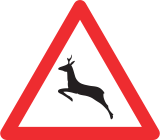
\includegraphics[width=0.7\linewidth]{imgs/16_real}
\end{subfigure}
\begin{subfigure}{.19\linewidth}
  \centering
  
\includegraphics[width=0.7\linewidth]{imgs/20_real}
\end{subfigure}
\caption{Submitted images}
\label{fig:test}
\end{figure}

\begin{enumerate}
\item
\textbf{Überholverbot für Kraftfahrzeuge aller Art: 99.99 \%}

The first adversarial example was generated from Git\-Hub's octocat using the Carlini \& Wagner L2 algorithm on a substitute model,
which was trained on the GTSRB training data.
It does not resemble the target sign at all and the source image is clearly recognizable.

\item
\textbf{Zulässige Höchstgeschwindigkeit (70): 99.41\%}

The second example was generated from the album cover of Pink Floyd's "The Dark Side of the Moon".
It uses the same setup as the first image.
Although there exists some noise on the black background, the target image is not recognizable and the album cover is still clearly visible.

\item
\textbf{Gefahrenstelle: $\approx$100\%}

\begin{figure}[!h]
\centering
\begin{subfigure}{.19\linewidth}
  \centering
  \includegraphics[width=0.7\linewidth]{imgs/robust_10/0_ll}
  \caption{99.97\%}
\end{subfigure}
\begin{subfigure}{.19\linewidth}
  \centering
  \includegraphics[width=0.7\linewidth]{imgs/robust_10/1_l}
  \caption{$\approx$100\%}
\end{subfigure}
\begin{subfigure}{.19\linewidth}
  \centering
  \includegraphics[width=0.7\linewidth]{imgs/robust_10/2_c}
  \caption{95.03\%}
\end{subfigure}
\begin{subfigure}{.19\linewidth}
  \centering
  \includegraphics[width=0.7\linewidth]{imgs/robust_10/3_r}
  \caption{99.85\%}
\end{subfigure}
\begin{subfigure}{.19\linewidth}
  \centering
  \includegraphics[width=0.7\linewidth]{imgs/robust_10/4_rr}
  \caption{99.98\%}
\end{subfigure}
\end{figure}

The third adversarial example is based on the GI logo.
It was constructed using the modified Carlini \& Wagner attack,
which modifies an image from multiple perspectives simultaneously.
The attack was performed on the model, which was trained using Jacobian based dataset augmentation.

The generated images are heavily perturbed;
yet, the GI logo is still noticeable while the target class is not recognizable.

\item
\textbf{Wildwechsel: 100\%}

\begin{figure}[!h]
\centering
\begin{subfigure}{.19\linewidth}
  \centering
  \includegraphics[width=0.7\linewidth]{imgs/robust_16/0_ll}
  \caption{97.62\%}
\end{subfigure}
\begin{subfigure}{.19\linewidth}
  \centering
  \includegraphics[width=0.7\linewidth]{imgs/robust_16/1_l}
  \caption{100\%}
\end{subfigure}
\begin{subfigure}{.19\linewidth}
  \centering
  \includegraphics[width=0.7\linewidth]{imgs/robust_16/2_c}
  \caption{100\%}
\end{subfigure}
\begin{subfigure}{.19\linewidth}
  \centering
  \includegraphics[width=0.7\linewidth]{imgs/robust_16/3_r}
  \caption{100\%}
\end{subfigure}
\begin{subfigure}{.19\linewidth}
  \centering
  \includegraphics[width=0.7\linewidth]{imgs/robust_16/4_rr}
  \caption{99.99\%}
\end{subfigure}
\end{figure}

The fourth adversarial example uses the same attack as the third, but is performed on the GTSRB-model.
It was generated from the Beatle's "Abbey Road" album cover.

Though the zebra crossing is still visible on closer inspection, the original image is too heavily perturbed to be identifiable. 
Nevertheless, the adversarial example does not resemble the target class (nor any other traffic sign) and is therefore valid.

\item
\textbf{Vorfahrt: 99.99\%}

The last image was created by the robust physical attack (RP$_2$) applied to the GTSRB-model.
It was generated from the logo of the three investigators (Die Drei Fragezeichen) where the question marks have been masked (i.e. they remain unperturbed).

\end{enumerate}

%!TEX root = paper.tex"`

\section{Model architecture}

\begin{enumerate}
\item Aufbau CNN\footnote{\url{https://chsasank.github.io/keras-tutorial.html}}

\begin{table}[!h]
\centering
\begin{tabular}{ l r }
\hline

Layer Type & GTSRB Model \\
\hline

  Convolution + ReLU & $3 \times 3 \times 32$ \\
  Convolution + ReLU & $3 \times 3 \times 32$  \\
  Max Pooling & $2 \times 2$ \\
  Dropout & $0.2$ \\

  Convolution + ReLU & $3 \times 3 \times 64$ \\
  Convolution + ReLU & $3 \times 3 \times 64$ \\
  Max Pooling & $2 \times 2$ \\
  Dropout & $0.2$ \\
  
  Convolution + ReLU & $3 \times 3 \times 128$ \\
  Convolution + ReLU & $3 \times 3 \times 128$ \\
  Max Pooling & $2 \times 2$ \\
  Dropout & $0.2$ \\
    
  Fully Connected + ReLU & $512$\\
  Dropout & $0.5$ \\

  Fully Connected + ReLU & $43$\\
  
  Softmax & $43$ \\ \hline 
  \vspace{1.5pt}
\end{tabular}
\caption{Architecture of our neural networks}
\label{table:model}
\end{table}
\item Geschichte Adversarial Samples
\item Carlini \& Wagner Angriff \cite{carlini2017towards}
\item Limitation of 64x64 -> no real world attack but constructed
\end{enumerate}

%!TEX root = paper.tex"`

\section{Evaluation}

To further evaluate the quality of the attacks, we generated multiple adversarial examples with different configurations and classified them using the \textbf{remote} model. 
In the following, we briefly discuss our setup and the selection of the attack parameters. Afterwards, we present and discuss the attack results.

\subsection{Setup}

\begin{table}
\begin{tabular}{l | l}
\textbf{Parameter} & \textbf{Values} \\\hline

target & 0,2,3,5,11,12,16,27,31,33 \\\hline

model & gtsrb\_model, jbda3\\\hline

attack & cwl2, robust\_cwl2\\\hline

image & abbey, gi, octocat\\\hline

conf & 15, 20
\end{tabular}
\caption{Attack Configuration}
\label{tab:cli_params}
\end{table}

\begin{minipage}{\linewidth}
An adversarial example is generated using the command line call:

\vspace{2ex}
\texttt{python3 attack\_model.py ----target [target]}

\hspace{4cm}\texttt{----model [model]}

\hspace{4cm}\texttt{----attack [attack]}

\hspace{4cm}\texttt{----image [image].png}

\hspace{4cm}\texttt{----confidence [conf]}

\hspace{4cm}\texttt{----max\_iterations 7500}

\hspace{4cm}\texttt{----binary\_search\_steps 12}
\vspace{2ex}
\end{minipage}

Arguments which are embraced by parentheses are taken from Table \ref{tab:cli_params}. 
If the Carlini \& Wagner attack (cwl2) is chosen as the attack technique, this attempts to create one adversarial example. 
Otherwise, if our modified Carlini \& Wagner attack (robust\_cwl2) is used, five adversarial examples are generated.\footnote{Please note, that the 'modified Carlini \& Wagner' attack from Section \ref{subsec:cwl2_mod} is internally referred to as robust\_cwl2} We omitted the Robust Physical Perturbation attack (RP$_2$) from our evaluation, because the success of the attack heavily depends on the masking image which might skew the results.

The attack\_model script only returns \emph{successful} adversarial examples, otherwise generating no image. 
For the Carlini \& Wagner attack, an adversarial example is successful if the local model classifies it as the target class. 
The modified Carlini \& Wagner attack only returns adversarial examples if the center image (where no perspective transformation is applied) is classified as the target class.

For our evaluation, we chose ten random labels as our target classes to keep the computation at a moderate level while still receiving meaningful results. 
The models under attack were created using the techniques from Section \ref{subsec:modelstealing}: \emph{Rebuilding} was used for the gtsrb model and \emph{Stealing} with Jacobian based dataset augmentation was used for the jbda model. 

The results of the attacks are displayed in Table \ref{tab:cwl2_result} and Table \ref{tab:robust_result}. 
Each cell shows the number of adversarial examples in the respective category. 
To illustrate this for the modified Carlini \& Wagner attack results (Table \ref{tab:robust_result}): 37 adversarial examples of the \enquote{abbey} image (which were generated with a confidence parameter of 20 against the gtsrb model) were classified with a confidence higher than 90\% by the remote model for the target class. 
On the other hand, four adversarial examples did not transfer and received a target-score lower than 90\%. 
Recall, that the modified C\&W attack is able to produce five adversarial example in one run. 
Therefore, the attack is potentially able to create 50 adversarial examples for the ten given targets. 
Thus, 43 of the potential 50 adversarial examples were successfully created on the local model.

In the following, we use the notation:

\begin{itemize}
\item[-] $P(C)$ = Probability of an adversarial example being successfully \textbf{created} on a local model
\item[-] $P(T)$ = Probability of an adversarial example \textbf{transferring} to the remote model (i.e. classification $\geq90\%$)
\item[-] $P(G)$ = Probability that the adversarial example was generated on the local \textbf{gtsrb model}
\item[-] $P(J)$ = Probability that the adversarial example was generated on the local \textbf{jbda model}
\end{itemize}

\subsection{Carlini \& Wagner}


\begin{table}
\begin{tabular}{l l | r r | r r | r r}
& & abbey & & gi & & octo & \\[1ex]
& & \footnotesize$\geq90\%$ & \footnotesize$<90\%$ & \footnotesize$\geq90\%$ & \footnotesize$<90\%$ & \footnotesize$\geq90\%$ & \footnotesize$<90\%$ \\[1ex]
\hline
gtsrb & 15 & 8 & 2 & 7 & 2 & 7 & 0 \\[1ex]
& 20 & 10 & 0 & 8 & 1 & 7 & 2 \\[1ex]
\hline
jbda & 15 & 6 & 3 & 1 & 3 & 6 & 1 \\[1ex]
& 20 & 7 & 0 & 2 & 3 & 6 & 1
\end{tabular}
\caption{Results for the Carlini \& Wagner attack}
\label{tab:cwl2_result}
\end{table}

The Carlini \& Wagner attack is fairly successful with a general probability of creating an adversarial example for the local model of

\begin{align*}
P(C) = \frac{93}{120} = 0.775
\end{align*}

Creating an adversarial image on the gtsrb model is far more likely than on the jbda model.

\begin{align*}
P(C \mid G) = \frac{54}{60} &= 0.9\\[1ex]
P(C \mid J) = \frac{39}{60} &= 0.65
\end{align*}

Additionally, it is more probable that the adversarial example transfers from the local model to the remote model, if it has been created on the gtsrb model:

\begin{align*}
P(T \mid G \wedge C) = \frac{47}{54} &\approx 0.87\\[1ex]
P(T \mid J \wedge C) = \frac{28}{39} &\approx 0.72
\end{align*}

Overall, it is far more likely to create a transferable image on the gtsrb model than on the jbda model. 

\begin{align*}
P(T \mid G) = \frac{47}{60} &\approx 0.78 \\[1ex]
P(T \mid J) = \frac{28}{60} &\approx 0.47
\end{align*}

\subsection{Modified Carlini \& Wagner}

\begin{table}
\begin{tabular}{l l | r r | r r | r r}
& & abbey & & gi & & octo & \\[1ex]
& & \footnotesize$\geq90\%$ & \footnotesize$<90\%$ & \footnotesize$\geq90\%$ & \footnotesize$<90\%$ & \footnotesize$\geq90\%$ & \footnotesize$<90\%$ \\[1ex]
\hline
gtsrb & 15 & 36 & 7 & 30 & 2 & 34 & 5
\\[1ex]
 & 20 & 37 & 4 & 30 & 4 & 38 & 5\\[1ex]
\hline
jbda & 15 & 30 & 7 & 12 & 3 & 26 & 8
\\[1ex]
  & 20 & 23 & 1 & 14 & 1 & 23 & 1
\end{tabular}
\caption{Results for the \textit{modified} Carlini \& Wagner attack}
\label{tab:robust_result}
\end{table}

The modified Carlini \& Wagner perturbs five transformations of the source image at the same time, which places additional constraints on the generation. This is visible in the overall reduced creation success of adversarial examples on the local model in comparison to the C\&W attack:

\begin{align*}
P(C) = \frac{381}{600} = 0.635
\end{align*}

Although the attack is still more likely to create adversarial examples on the gtsrb model than on the jbda model, its probability is noticeably reduced:

\begin{align*}
P(C \mid G) = \frac{232}{300} &\approx 0.77\\[1ex]
P(C \mid J) = \frac{149}{300} &\approx 0.50
\end{align*}

However, the transferability of adversarial examples, which have been successfully created on a local model, increased for the jbda model and are unchanged for the gtsrb model. Thus, images created on either model have approximately the same probability of transferring to the remote model:

\begin{align*}
P(T \mid G \wedge C) = \frac{205}{232} &\approx 0.88\\[1ex]
P(T \mid J \wedge C) = \frac{128}{149} &\approx 0.86
\end{align*}

Overall, the gtsrb model is preferable over the jbda model for creating transferable adversarial examples in both attacks. 

\begin{align*}
P(T \mid G) = \frac{205}{300} &\approx 0.68\\[1ex]
P(T \mid J) = \frac{128}{300} &\approx 0.43
\end{align*}

To us this is quite surprising, because the jbda model used the Jacobian-based dataset augmentation for training, which is a far more sophisticated technique than the simple dataset training of the gtsrb model. 
Although the Jacobian-based dataset augmentation did not work perfectly well (it achieved a top validation accuracy of about 86\% on the remotely fetched labels), we would have expected it to better approximate the remote model.
That a more simple approach however performs better is especially remarkable as multiple classes are missing from the remote model's predictions -- as we discussed in Section \ref{subsec:modelstealing} -- and we had assumed, that this would hinder a favorable rebuilding of the remote model's decision boundary.

%!TEX root = paper.tex"`

\section{Extensibility}

\begin{enumerate}
\item Weitere Angriffe einbauen
\item Eigene Maske bei Physical-Attack durch Benutzer definieren
\item Mehrbenutzersystem
\item ...
\end{enumerate}

%\bibliographystyle{IEEEtran}
%TODO find source of szegedy2013 other than arXiv
\bibliographystyle{plainnat}
\bibliography{bib} %name of bib file

%!TEX root = paper.tex
\clearpage
\appendix
\section{Process Management with Double-Fork}\label{app:doublefork}
\begin{figure}[H]\label{fig:process_sequence}
	\centering
	\begin{subfigure}{1.2\linewidth}
		\centering
		\includegraphics[width=1.2\linewidth]{figs/process_sequence}
	\end{subfigure}
	\caption{The sequence of internal requests to start a process and poll its status.}
\end{figure}
\end{document}
